\chapter{Fallstudie}\label{ch:Fallstudie}
\paragraph{Szenario}
Für unseren Online-Shop soll eine neue Benutzerverwaltung entwickelt werden, nachdem die alte nicht mehr Wartbar ist. Dazu zählt das Anmelden und neu registrieren von Nutzern wie auch das ausgeben der Benutzerdaten zu einem Nutzer.

\paragraph{Gründe für einen Microservice}
Da man aus den Problemen der vorherigen Benutzerverwaltung lernt, soll die neue Verwaltung auch langfristig Wartbar bleiben. \newline
Auch soll jedes Teilgebiet der Anwendung von einem einzelnen Team umgesetzt werden. Dabei hat jedes Team andere Präferenzen welche Technologie genutzt werden soll. So möchte ein Team bei den alt bewährten Technologien bleiben und entwicklet in Java. Ein Anderes Team möchte sich in neuere Technologien einarbeiten und versucht ihren Microservice mit Webtechnologien umzusetzen. \newline
Ein weiterer Grund für die Nutzung ist die erleichterte Integration neuer Systeme sowie die Integration in ein anderes System. Gerade im Falle einer Benutzeranmeldung, die in mehreren Systemen zum Einsatz kommen kann. Je nach System können die hier entwickelten Grundbausteine erhalten bleiben und neue Funktionen mit weiteren Microservices hinzugefügt werden.

\paragraph{Planung}

Wir sind folgendermaßen vorgegangen: Zuerst haben wir geplant wie unser beispielhaftes Microservice -System aussehen soll. Dabei haben wir uns auf ein Login-System festgelegt, da dieses Szenario einen großen Anwendungsbezug hat - auf fast jeder Webseite befindet sich ein Anmeldesystem. \newline
Um möglichst viele Aspekte von Micorservices zu erfahren und aufzeigen zu können haben wir uns dafür entscheiden, möglichst kleine Micorservices zu planen. Das bedeutet: ein einem realen System wären die unterschiedlichen Funktionen wahrscheinlich in einem Service zusammengefasst, in diesem Beispiel sind diese aus Anschauungsgründen jedoch in unterschiedlichen Microservices. \newline
Schon an diesem kleinen Beispiel kann ist erkennbar, dass die Planung der Architektur der Schwierig ist, da wir uns auch schon bei der Einteilung der Services nicht immer sicher waren wie etwas am Besten aufzuteilen und umzusetzen ist. Bei größeren Systemen wäre dieses Problem um Längen schwerer zu lösen. \newline
Nachdem die einzelnen Services den Teams/Personen  zugeordnet waren, wurden diese völlig voneinander getrennt entwickelt. Wir haben keine Technologie vorausgesetzt und jeder durfte für sich entscheiden, was er als am sinnvollsten hielt bzw. worin die Person Erfahrung sammeln wollte. \newline
Bei der Architektur haben wir uns dafür entschieden die Backendservices, die auf die Datenbanken zugreifen, von der Benutzeroberfläche zu trennen. Dadurch hatten wir mehr Flexibilität bezüglich Ausführbarkeit der Oberfläche im Browser.

\paragraph{Durchführung}
Nach dem Aufteilen der Services hat jeder für sich die Services entwickelt ohne dass dafür zusätzliche Absprachen benötigt wurden. So wurde die Benutzeroberfläche mit Typescript und React.js als Webapp im Material Design entwickelt. Der Microservice zum Registrieren neuer Nutzer wurde mittels Java umgesetzt. Die Services zum anzeigen aller Daten und zum anmelden läuft auf node.js und wurde in Typescript geschrieben. Für die Datenbanken wurde zwei mal MySQL benutzt, was jedoch nicht abgesprochen war. Die Kommunikation zwischen den Microservices läuft, wie es auch in vielen größeren Microservice-Systemen üblich ist, über http und basiert auf REST. \newline
Es ist erkennbar wie die Wahl der Technologien bei der Entwicklung keine Rolle gespielt hat und neue Sprachen ausprobiert werden konnten.

\begin{figure}[bth] 
	\centering
	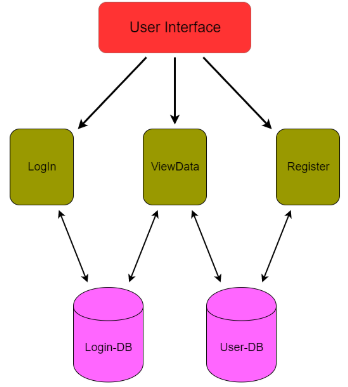
\includegraphics[width=0.7\textwidth]{Chapters/Bilder/Architektur}
	\caption{Die Architektur der Fallstudie}
	\label{fig:Architektur}
\end{figure}


\paragraph{Funktionsweise}
In der \textbf{User-DB} sind die Daten zu den Nutzern gespeichert wie Nutzername, Email und Passwort. Zum identifizieren der Nutzer wird jedem Nutzer eine ID zugewiesen die ebenfalls in dieser Datenbank gespeichert wird. Diese Daten werden von dem \textbf{Register} Microservice geschrieben, sobald sich ein Nutzer registriert. \newline
Gelesen werden diese Daten vom \textbf{ViewData} Microservice, wenn dem Nutzer seine gesamten Daten angezeigt werden. Dazu zählen ebenfalls Daten aus der Login-DB. \newline
In der \textbf{Login-DB} wird gespeichert, ob ein Nutzer derzeit angemeldet ist. Beim anmelden genereirt der \textbf{LogIn} Microservice ein Token, welches in der Datenbank gespeichert wird und ebenfalls dem Nutzer zurückgegeben wird. In der Datenbank wird dem Nutzer das Token mittels der ID zugeordnet. \newline
Mit diesem Token kann der Nutzer den \textbf{ViewData} Microservice aufrufen der zu dem Nutzer die Daten ausgibt (inclusive ID und Token aus Login-DB). \newline
Die gesamte Steuerung kann der Nutzer über die Benutzeroberfläche einfach und intuitiv vornehmen. Dazu gibt es 3 Verschiedene Ansichten. 
\begin{figure}[bth]
	\subfloat[Registirerung]{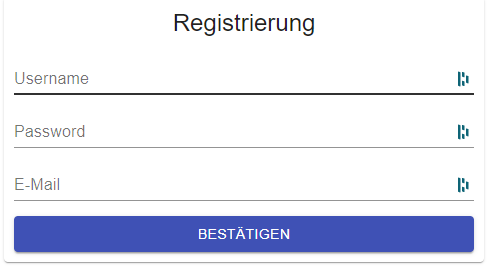
\includegraphics[width=0.40\textwidth]{Chapters/Bilder/ViewRegister}\label{subfig:ViewRegister}}\hfill
	\subfloat[Anmeldung]{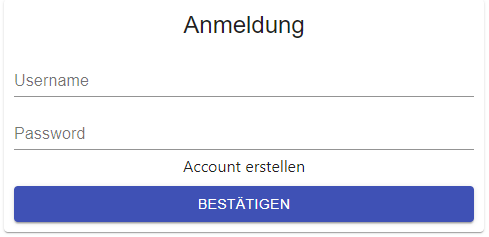
\includegraphics[width=0.40\textwidth]{Chapters/Bilder/ViewLogIn}\label{subfig:ViewLogIn}}
	\subfloat[Datenausgabe]{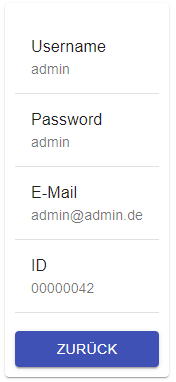
\includegraphics[width=0.20\textwidth]{Chapters/Bilder/ViewViewData}\label{subfig:abbtwo}}
	\caption{Die Benutzeroberfläche}
	\label{fig:UI}
\end{figure}

\paragraph{Herausforderung}
Beim Entwicklungsprozess sind uns selbst ein einem so kleinen und primitiven Projekt viele der Herausforderungen aufgefallen. So ist uns das sinnvolle Aufteilen der Funktionen und Datenbanken schwer gefallen. Bei großen Projekten ist dies wahrscheinlich exponentiell komplexer. \newline
Auch wäre eine realistische Infrastruktur aufgrund des Initalen Administrationsaufwandes nicht möglich gewesen (Router konfigurieren, pro Micorservice eine VM aufsetzen ...).

